\documentclass{article}
\usepackage[margin=0.9in]{geometry}
\usepackage{graphicx} % Required for inserting images
\usepackage{amssymb}
\usepackage{amsmath}
\usepackage{amsthm}
\usepackage{tikz}
\usepackage{stanli}
\usetikzlibrary {arrows.meta, bending}

\title{Introduction to Finite Elements and Algorithms}
\author{Group 3}
\date{November 2023}


\begin{document}

\maketitle

\section{Poisson Equation 2D}

Many physical phenomena can be modeled with the Poisson Equation.

\begin{equation}\label{eq:2D_Poisson}
    \nabla\left(\kappa\nabla u \right) +\alpha u= f(x,y) \qquad \forall x,y\in \Omega
\end{equation}

With boundary conditions:

\begin{equation}\label{eq:2D_PoissonBC}
    \begin{gathered}
        q \quad \text{on} \quad \Gamma_{N} \\
        T \quad \text{on} \quad \Gamma_{D}  \\ 
        \Gamma_{N} \cup \Gamma_{D} = \partial \Omega \\
        \Gamma_{N} \cap \Gamma_{D} = {0}
    \end{gathered}    
\end{equation}

We multiplicate or function with a test function $v$. And integrate over the domain. 

\begin{equation}\label{eq:2D_PoissonInt}
    \begin{gathered}
        \left(\nabla\left(\kappa\nabla u \right)+\alpha u\right) v  = f(x,y) v \qquad \forall x,y\in \Omega \\
        \int_{\Omega}{\left(\nabla\left(\kappa\nabla u \right)+\alpha u\right) v d\Omega}=\int_{\Omega}{f(x,y) v d\Omega} \qquad \forall x,y\in \Omega \\
    \end{gathered}
\end{equation}

Using Green's theorem, we can change the divergence operator to the test function $v$.

\begin{equation}\label{eq:2D_Poisson_Weak}
    \begin{gathered}
        \int_{\partial\Omega}{\left(\kappa\nabla u \cdot\textbf{n}_t\right) v d\Omega}-\int_{\Omega}{\kappa\nabla u  \nabla v d\Omega}+\int_{\Omega}{\alpha u v d\Omega}=\int_{\Omega}{f(x,y) v d\Omega}\\
    \end{gathered}
\end{equation}

Now, we discretize the domain into different elements $\Omega^e$, the field on each element is approximate with shape functions $\varphi_i(x,y)$. The test function is selected to be the same as the shape function $\varphi_j(x,y)$ (Galerkin Formulation). For the following analysis, we will forget about the boundary conditions, which will be applied in the last steps of the formulation.

\begin{equation}\label{eq:2D_Poisson_Dis}
    \begin{gathered}
        \tilde{u}\approx\sum_{i=1}^{n}{u_i\varphi_i}\\
        -\int_{\Omega^e}{\kappa(\nabla \tilde{u})  (\nabla \varphi_j ) d\Omega^e}+\int_{\Omega^e}{\alpha \tilde{u} \varphi_j  d\Omega^e}=\int_{\Omega}{f(x,y) \varphi_j d\Omega^e}\\
        \nabla \tilde{u}=\nabla\left(\sum_{i=1}^{n}{u_i\varphi_i}\right)=\sum_{i=1}^{n}{u_i\nabla(\varphi_i)}\\
        -\int_{\Omega^e}{\kappa\left(\sum_{i=1}^{n}{u_i\nabla(\varphi_i)}\right)  (\nabla \varphi_j ) d\Omega^e}+\int_{\Omega^e}{\alpha\left(\sum_{i=1}^{n}{u_i\varphi_i}\right)\varphi_j d\Omega^e}=\sum_{i=1}^{n}{\left(\int_{\Omega^e}{\alpha \varphi_i \varphi_j d\Omega^e}-\int_{\Omega^e}{\kappa (\nabla\varphi_i)  (\nabla \varphi_j ) d\Omega^e}\right)u_i}\\
        \sum_{i=1}^{n}{\left(\int_{\Omega^e}{\alpha \varphi_i \varphi_j d\Omega^e}-\int_{\Omega^e}{\kappa (\nabla\varphi_i)  (\nabla \varphi_j ) d\Omega^e}\right)u_i}=\int_{\Omega}{f(x,y) \varphi_j d\Omega^e} 
    \end{gathered}
\end{equation}

For each element, we have $n$ unknowns but only one equation. To get the missing $n-1$ equations, we vary the index $j=1,2..,n$ to get a linear equation system.

\begin{equation}\label{eq:2D_Poisson_Sys}
    \begin{gathered}
        (-\textbf{S}+\textbf{M})u=f\\
        \textbf{S}=[S_{ij}]=\int_{\Omega^e}{\kappa (\nabla\varphi_i)  (\nabla \varphi_j ) d\Omega^e}\\
        \textbf{M}=[M_{ij}]=\int_{\Omega^e}{\alpha \varphi_i \varphi_j d\Omega^e}\\
        u=[u_i]=u_i\\
        f=[f_i]=\int_{\Omega}{f(x,y) \varphi_j d\Omega^e}
    \end{gathered}
\end{equation}

$S$ is the element stiffness matrix, $u$ is the unknown vector, and $f$ is the element force vector.

If we discretize our domain in linear triangular elements, we will need to use natural coordinates to have a general formulation of the local matrices and vectors.

\begin{figure}[h]
    \centering
    \begin{tikzpicture}
      % Define the vertices of the triangle
      \coordinate (A) at (1,2);
      \coordinate (B) at (4,3);
      \coordinate (C) at (2,3);
    
      % Draw the triangle
      \draw[line width=1.5pt] (A) -- (B) -- (C) -- cycle;
    
      % Label the vertices
      \node[below] at (A) {$P_1$};
      \node[below] at (B) {$P_2$};
      \node[above] at (C) {$P_3$};

      % Draw coordinate axes
      \draw[->] (-1,0) -- (5,0) node[right] {$x$};
      \draw[->] (0,-1) -- (0,4) node[above] {$y$};
    \end{tikzpicture}
    \caption{Triangular Element}
    \label{fig:global_Tria}
\end{figure}

Where $x_i$ and $y_i$ are the coordinates of the point $P_i$. We transform this element to the following natural coordinates.


\begin{figure}[h]
    \centering
    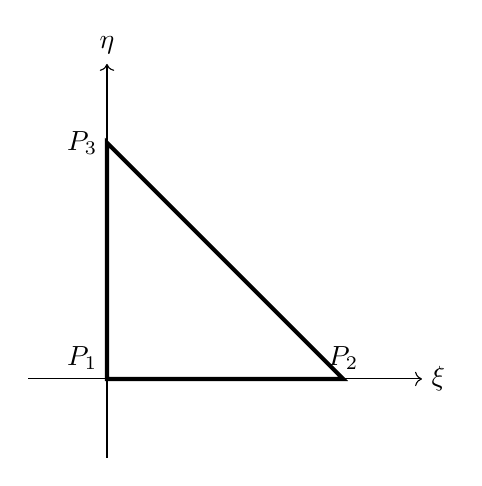
\begin{tikzpicture}
      % Define the vertices of the triangle
      \coordinate (A) at (0,0);
      \coordinate (B) at (3,0);
      \coordinate (C) at (0,3);
    
      % Draw the triangle
      \draw[line width=1.5pt] (A) -- (B) -- (C) -- cycle;
    
      % Label the vertices
      \node[above left] at (A) {$P_1$};
      \node[above] at (B) {$P_2$};
      \node[left] at (C) {$P_3$};

      % Draw coordinate axes
      \draw[->] (-1,0) -- (4,0) node[right] {$\xi$};
      \draw[->] (0,-1) -- (0,4) node[above] {$\eta$};
    \end{tikzpicture}
    \caption{Triangular Element}
    \label{fig:local_Tria}
\end{figure}

The shape functions used for this element are linear Lagrange functions.

\begin{equation}\label{eq:SF_t}
    \begin{gathered}
        \varphi_1(\xi,\eta)=1-\xi-\eta\\
        \varphi_2(\xi,\eta)=\xi\\
        \varphi_3(\xi,\eta)=\eta
    \end{gathered}
\end{equation}

And using an isoparametric approach, we can describe the geometry.

\begin{equation}\label{eq:x_t}
    \begin{gathered}
        x=\varphi_1x_1+\varphi_2x_2+\varphi_3x_3\\
        y=\varphi_1y_1+\varphi_2y_2+\varphi_3y_3
    \end{gathered}
\end{equation}

The matrices in local coordinates should be the following.

\begin{equation}\label{eq:2D_Poisson_Sys}
    \begin{gathered}
        \nabla \varphi_i=\frac{\partial\varphi_i}{\partial x}+\frac{d\varphi_i}{\partial y}\\
        \frac{\partial \varphi_i}{\partial x}=\frac{\partial\varphi_i}{\partial\xi}\frac{\partial\xi}{\partial x}+\frac{d\varphi_i}{\partial\eta}\frac{\partial\eta}{\partial x}\\
        \frac{\partial\varphi_i}{\partial y}=\frac{\partial\varphi_i}{\partial\xi}\frac{\partial\xi}{\partial y}+\frac{d\varphi_i}{d\eta}\frac{d\eta}{\partial y}\\
        dx=\frac{\partial x}{\partial\xi}d\xi+\frac{\partial x}{d\eta}d\eta\\
        dy=\frac{dy}{d\xi}d\xi+\frac{dy}{d\eta}d\eta\\
        \textbf{J}=\begin{bmatrix}
            \frac{\partial x}{\partial \xi} & \frac{\partial y}{\partial \xi}\\
            \frac{\partial x}{\partial \eta} & \frac{\partial y}{\partial \eta}
        \end{bmatrix}\\
        \textbf{J}^{-1}=\begin{bmatrix}
            \frac{\partial \xi}{\partial x} & \frac{\partial \eta}{\partial x}\\
            \frac{\partial \eta}{\partial x} & \frac{\partial \eta}{\partial \xi}
        \end{bmatrix}\\
        \begin{bmatrix}
            \frac{\partial \varphi_i}{\partial x}\\
            \frac{\partial \varphi_i}{\partial y}
        \end{bmatrix}
        =\textbf{J}^{-1}\begin{bmatrix}
            \frac{\partial \varphi_i}{\partial \xi}\\
            \frac{\partial \varphi_i}{\partial \eta}
        \end{bmatrix} \\
    \end{gathered}
\end{equation}

The derivatives of the shape functions in local coordinates are the following:

\begin{equation}\label{eq:SF_t}
    \begin{gathered}
        \frac{\partial \varphi_1}{\partial \xi}=-1\\
        \frac{\partial \varphi_1}{\partial \eta}=-1\\
        \frac{\partial \varphi_2}{\partial \xi}=1\\
        \frac{\partial \varphi_2}{\partial \eta}=0\\
        \frac{\partial \varphi_3}{\partial \xi}=0\\
        \frac{\partial \varphi_3}{\partial \eta}=1\\
    \end{gathered}
\end{equation}

The global coordinates variables are:

\begin{equation}\label{eq:SF_t}
    \begin{gathered}
        \frac{\partial x}{\partial \xi}=-x_1+x_2\\
        \frac{\partial x}{\partial \eta}=-x_1+x_3\\
        \frac{\partial y}{\partial \xi}=-y_1+y_2\\
        \frac{\partial y}{\partial \eta}=-y_1+y_3\\
        \textbf{J}=\begin{bmatrix}
            x_2-x_1&y_2-y_1 \\
            x_3-x_1&y_3-y_1
        \end{bmatrix}\\
        \textbf{J}^{-1}= \frac{1}{(x_2-x_1)(y_3-y_1) - (x_3-x_1)(y_2-y_1)} \begin{bmatrix}
y_3-y_1 & -(y_2-y_1) \\
-(x_3-x_1) & x_2-x_1
\end{bmatrix}\\
\begin{bmatrix}
    1 & 1
\end{bmatrix}\textbf{J}^{-1}=\frac{1}{(x_2-x_1)(y_3-y_1) - (x_3-x_1)(y_2-y_1)}\begin{bmatrix} (y_3-y_1) - (x_3-x_1) & -(y_2-y_1) + (x_2-x_1) \end{bmatrix}\\
\begin{bmatrix}
    1 & 1
\end{bmatrix}\textbf{J}^{-1}\begin{bmatrix}
            \frac{\partial \varphi_1}{\partial \xi}\\
            \frac{\partial \varphi_1}{\partial \eta}
        \end{bmatrix} =\frac{  - y_3 + x_3 + y_2 - x_2}{(x_2-x_1)(y_3-y_1) - (x_3-x_1)(y_2-y_1)}\\
        \begin{bmatrix}
    1 & 1
\end{bmatrix}\textbf{J}^{-1}\begin{bmatrix}
            \frac{\partial \varphi_2}{\partial \xi}\\
            \frac{\partial \varphi_2}{\partial \eta}
        \end{bmatrix} =\frac{ y_3 - y_1 - x_3 + x_1}{(x_2-x_1)(y_3-y_1) - (x_3-x_1)(y_2-y_1)}\\
        \begin{bmatrix}
    1 & 1
\end{bmatrix}\textbf{J}^{-1}\begin{bmatrix}
            \frac{\partial \varphi_3}{\partial \xi}\\
            \frac{\partial \varphi_3}{\partial \eta}
        \end{bmatrix} =\frac{ -y_2 + y_1 + x_2 - x_1}{(x_2-x_1)(y_3-y_1) - (x_3-x_1)(y_2-y_1)}
    \end{gathered}
\end{equation}

The system 0f equations in local coordinates will be then:

\begin{equation}\label{eq:2D_Poisson_Sys}
    \begin{gathered}
        \textbf{S}=[S_{ij}]=\int_{\Omega^{l}}{\kappa \left(\begin{bmatrix}
            1&1
        \end{bmatrix}\textbf{J}^{-1}\begin{bmatrix}
            \frac{\partial \varphi_i}{\partial \xi}\\
            \frac{\partial \varphi_i}{\partial \eta}
        \end{bmatrix}   \right)\left(\begin{bmatrix}
            1&1
        \end{bmatrix}\textbf{J}^{-1}\begin{bmatrix}
            \frac{\partial \varphi_j}{\partial \xi}\\
            \frac{\partial \varphi_j}{\partial \eta}
        \end{bmatrix}   \right) |det(\textbf{J})|d\xi d\eta}\\
        \textbf{M}=[M_{ij}]=\int_{\Omega^l}{\alpha \varphi_i \varphi_j |det(\textbf{J})|d\xi d\eta}\\
        u=[u_i]=u_i\\
        f=[f_i]=\int_{\Omega^l}{f(x(\xi,\eta),y(\xi,\eta)) \varphi_j |det(\textbf{J})|d\xi d\eta}
    \end{gathered}
\end{equation}

\end{document}
